\documentclass{standalone}
\usepackage{tikz}
\usepackage{ctex,siunitx,ninecolors}
\setCJKmainfont{Noto Serif CJK SC}
\usepackage{tkz-euclide}
\usepackage{amsmath}
\usetikzlibrary{patterns, calc}
\usetikzlibrary {decorations.pathmorphing, decorations.pathreplacing, decorations.shapes}
\begin{document}
\small
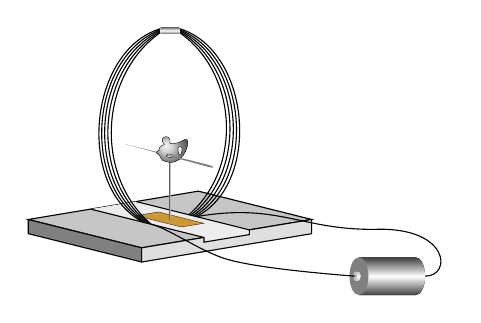
\begin{tikzpicture}[scale=1.2]
  \begin{scope}[scale=1.5]
  \draw[fill=lightgray!90](-1,0)--(0.2,0.2)--(1,0)--(-0.2,-0.2)--cycle;
  \draw[fill=gray](-1,0)--(-1,-0.1)--(-0.2,-0.3)--(-0.2,-0.2)--cycle;
  \draw[fill=lightgray!50](-0.2,-0.2)--(-0.2,-0.3)--(1,-0.1)--(1,0)--cycle;
  \end{scope}
  \draw[fill=lightgray!30](-0.84,0.11)--(0.36,-0.19)--(0.36,-0.24)--(0.84,-0.16)--(0.84,-0.11)--(-0.36,0.19);
  \foreach \x/\y/\z/\a in {0.24/0.04/2.0/60,0.22/0.045/1.99/56,0.2/0.05/1.98/52,0.26/0.035/2.01/64,0.28/0.03/2.02/68}
  {
    \draw(\x,\y)to[bend right=\a](0.1,\z);
  }
  \begin{scope}[xscale=-0.4,yscale=0.4]
  \draw[fill=brown!80!yellow,ultra thin](0.9,0.1)--(-0.3,-0.2)--(-0.9,-0.1)--(0.3,0.2)--cycle;
  \fill[left color=gray,right color=gray,middle color=white](-0.02,0)arc(180:360:0.02 and 0.01)--(0.02,1.6)--(-0.02,1.6)--cycle;
  \fill[gray](1.2,2)--(0,1.7)--(0,1.67)--cycle;
  \fill[ball color=lightgray,draw=black,ultra thin]( 0.145,1.985)..controls( 0.373,1.885)and( 0.222,1.897)..
  ( 0.299,1.833)..controls( 0.330,1.812)and( 0.405,1.773)..
  ( 0.316,1.724)..controls( 0.222,1.667)and( 0.275,1.600)..
  ( 0.194,1.565)..controls(-0.315,1.329)and(-0.519,1.952)..
  (-0.461,2.097)..controls(-0.445,2.142)and(-0.343,2.101)..
  (-0.289,2.064)..controls(-0.198,2.011)and(-0.094,2.008)..
  (-0.046,2.007)..controls(-0.035,2.009)and(-0.005,1.999)..
  ( 0.003,2.020)..controls( 0.012,2.049)and( 0.000,2.050)..
  (-0.001,2.104)..controls(-0.002,2.249)and( 0.252,2.203)..
  ( 0.204,2.067)..controls( 0.179,2.011)and( 0.174,2.031)..cycle
  (-0.214,1.901)..controls(-0.369,1.987)and(-0.316,1.814)..
  (-0.297,1.732)..controls(-0.205,1.671)and(-0.216,1.829)..cycle
  ( 0.101,1.681)..controls( 0.121,1.794)and(-0.209,1.704)..
  (-0.044,1.646)..controls( 0.007,1.631)and( 0.097,1.635)..cycle;
  \fill[gray](0,1.7)--(-1,1.45)..controls(-1.2,1.4)and(-1.2,1.34)..(-1,1.395)--(0,1.67);
  \end{scope}
  \foreach \x/\y/\z/\a in {-0.24/-0.04/2.0/60,-0.22/-0.045/1.99/56,-0.2/-0.05/1.98/52,-0.26/-0.035/2.01/64,-0.28/-0.03/2.02/68}
  {
    \draw(\x,\y)to[bend left=\a](-0.1,\z);
  }
  \fill[top color=gray,bottom color=gray,middle color=white](-0.1,1.97)rectangle(0.1,2.03);
  \fill[top color=darkgray,bottom color=darkgray,middle color=white](2.0,-0.8)--(2.6,-0.8)arc(-90:90:0.1 and 0.2)--(2.0,-0.4)--cycle;
  \fill[gray](2.0,-0.6)ellipse(0.1 and 0.2);
  \fill[top color=lightgray,bottom color=lightgray,middle color=white](1.96,-0.65)--(2.0,-0.65)arc(-90:90:0.02 and 0.05)--(1.96,-0.55)--cycle;
  \fill[lightgray](1.96,-0.6)ellipse(0.02 and 0.05);
  \draw(-0.200,-0.050)..controls( 0.000,-0.100)and( 0.313,-0.334)..
  ( 0.607,-0.422)..controls( 0.802,-0.478)and( 1.213,-0.542)..( 1.960,-0.600)
  ( 0.280, 0.030)..controls( 1.151, 0.181)and( 1.388,-0.117)..
  ( 2.186,-0.104)..controls( 2.962,-0.083)and( 2.986,-0.600)..(2.70,-0.600);
\end{tikzpicture}
\end{document}